\documentclass{standalone}
\usepackage{tikz}
\usetikzlibrary{patterns, positioning}
\usepackage[sfdefault]{ClearSans} %% option 'sfdefault' activates Clear Sans as the default text font
\usepackage[T1]{fontenc}

\begin{document}
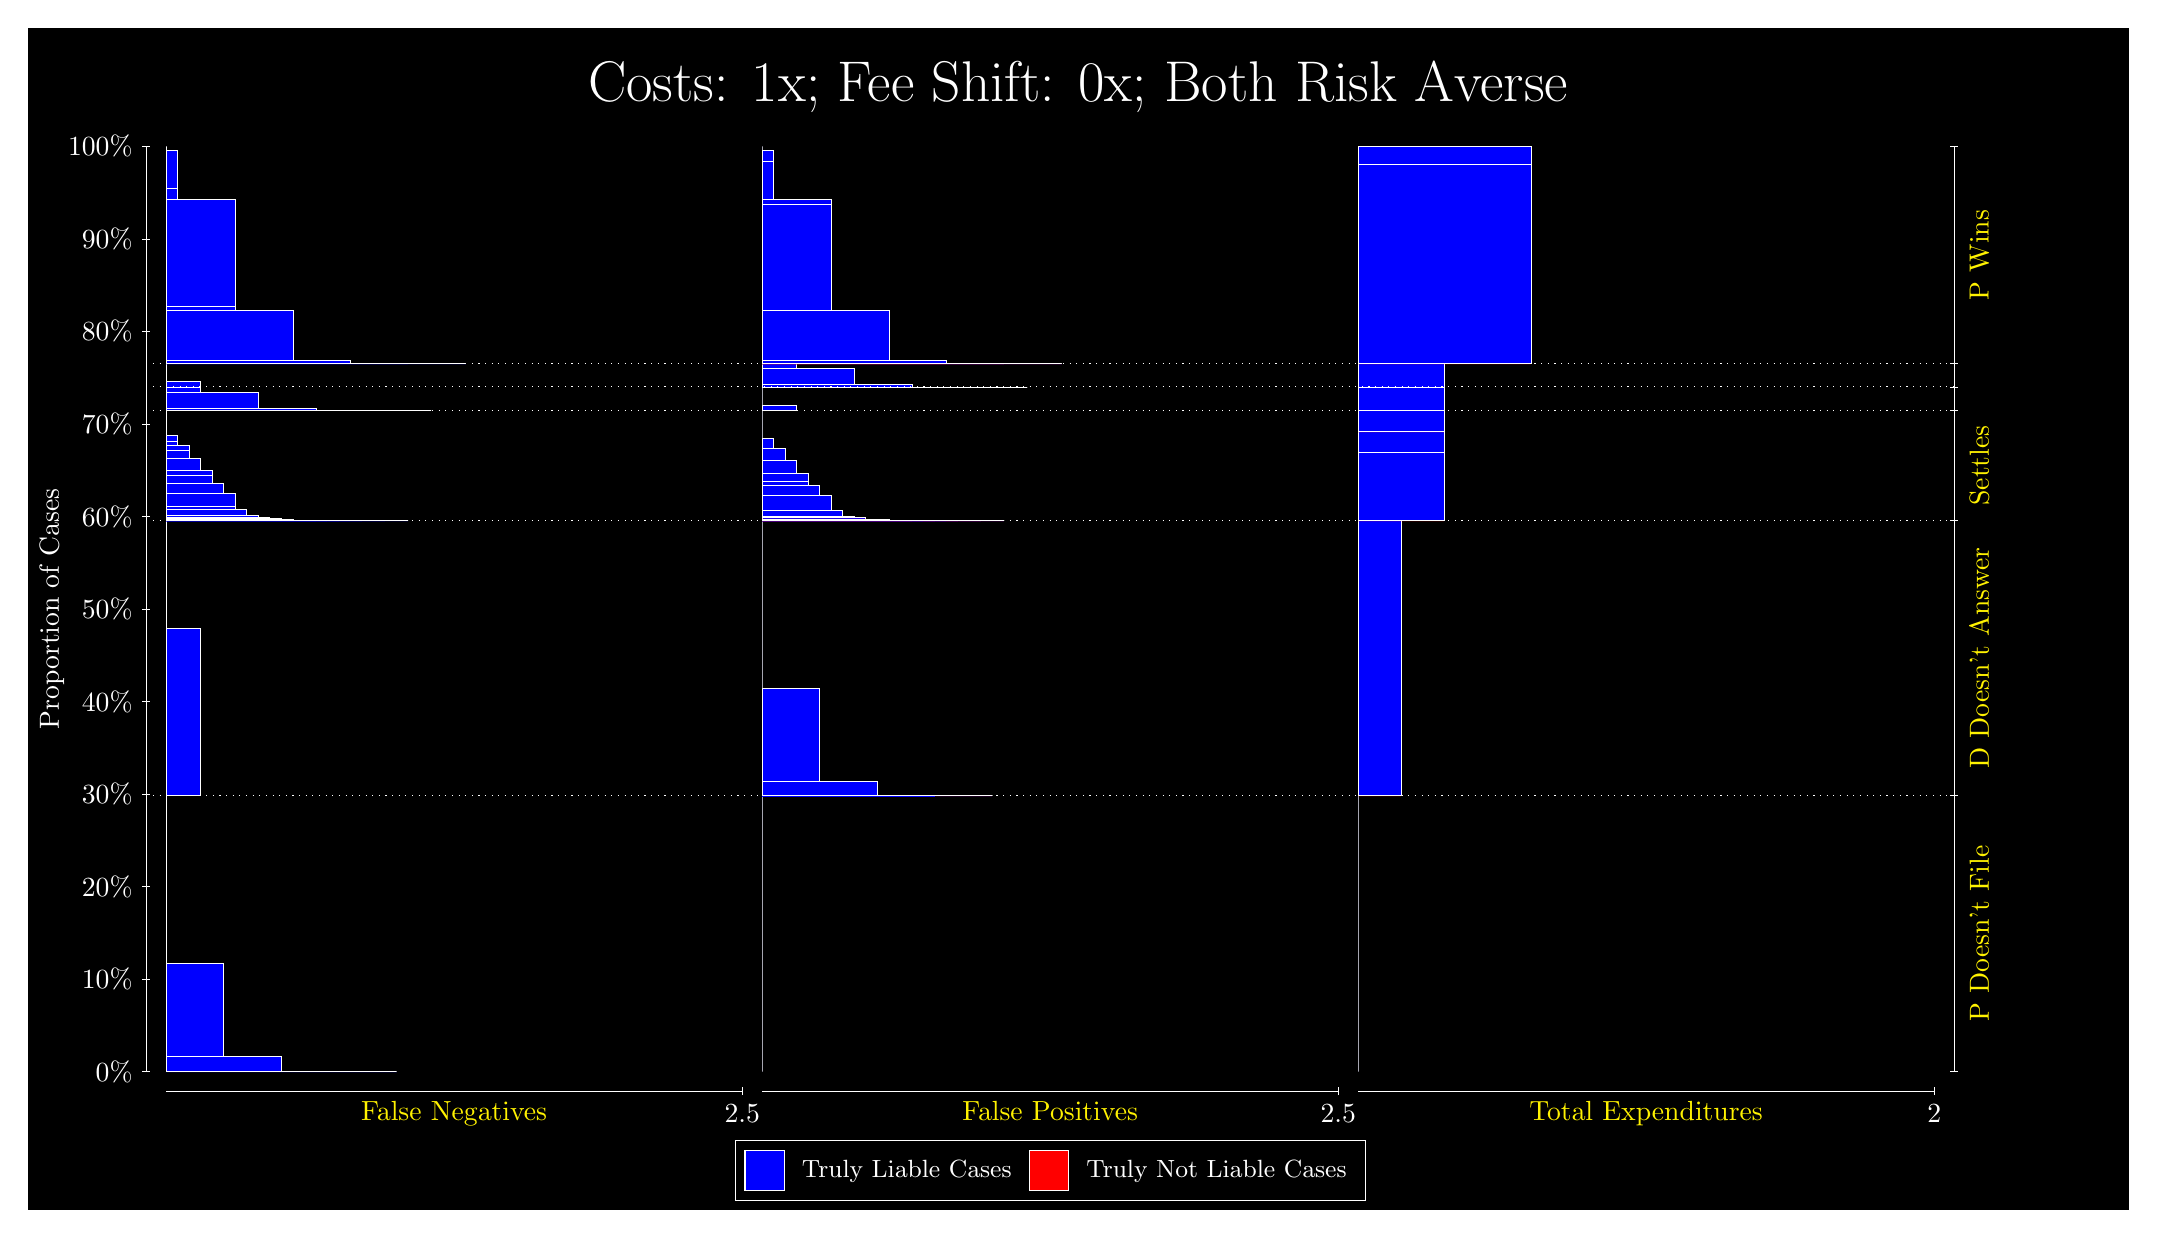
\begin{tikzpicture}
\draw[fill=black] (0,0) rectangle (26.667,15);
\draw[text=white] (0,13.5) rectangle (26.667,15) node[midway] {\huge Costs: 1x; Fee Shift: 0x; Both Risk Averse};
\draw[white, very thin] (1.5,1.75) -- (1.5,13.5);
\node[rotate=90, text=white, anchor=center] at (0.3, 7.625) {Proportion of Cases};
\draw[white, very thin] (1.45,1.75) -- (1.55,1.75);
\node[text=white, anchor=east] at (1.45, 1.75) {0\%};
\draw[white, very thin] (1.45,2.925) -- (1.55,2.925);
\node[text=white, anchor=east] at (1.45, 2.925) {10\%};
\draw[white, very thin] (1.45,4.1) -- (1.55,4.1);
\node[text=white, anchor=east] at (1.45, 4.1) {20\%};
\draw[white, very thin] (1.45,5.275) -- (1.55,5.275);
\node[text=white, anchor=east] at (1.45, 5.275) {30\%};
\draw[white, very thin] (1.45,6.45) -- (1.55,6.45);
\node[text=white, anchor=east] at (1.45, 6.45) {40\%};
\draw[white, very thin] (1.45,7.625) -- (1.55,7.625);
\node[text=white, anchor=east] at (1.45, 7.625) {50\%};
\draw[white, very thin] (1.45,8.8) -- (1.55,8.8);
\node[text=white, anchor=east] at (1.45, 8.8) {60\%};
\draw[white, very thin] (1.45,9.975) -- (1.55,9.975);
\node[text=white, anchor=east] at (1.45, 9.975) {70\%};
\draw[white, very thin] (1.45,11.15) -- (1.55,11.15);
\node[text=white, anchor=east] at (1.45, 11.15) {80\%};
\draw[white, very thin] (1.45,12.325) -- (1.55,12.325);
\node[text=white, anchor=east] at (1.45, 12.325) {90\%};
\draw[white, very thin] (1.45,13.5) -- (1.55,13.5);
\node[text=white, anchor=east] at (1.45, 13.5) {100\%};

\draw[white, very thin] (24.457,1.75) -- (24.457,13.5);
\draw[white, very thin] (24.407,1.75) -- (24.507,1.75);
\node[anchor=west] at (24.407, 1.75) {};
\draw[white, very thin] (24.407,5.2547) -- (24.507,5.2547);
\node[anchor=west] at (24.407, 5.2547) {};
\draw[white, very thin] (24.407,8.7469) -- (24.507,8.7469);
\node[anchor=west] at (24.407, 8.7469) {};
\draw[white, very thin] (24.407,10.145) -- (24.507,10.145);
\node[anchor=west] at (24.407, 10.145) {};
\draw[white, very thin] (24.407,10.445) -- (24.507,10.445);
\node[anchor=west] at (24.407, 10.445) {};
\draw[white, very thin] (24.407,10.741) -- (24.507,10.741);
\node[anchor=west] at (24.407, 10.741) {};
\draw[white, very thin] (24.407,13.5) -- (24.507,13.5);
\node[anchor=west] at (24.407, 13.5) {};

\draw[white, very thin, fill=blue] (1.75,1.75) rectangle (4.6775,1.75);
\draw[white, very thin, fill=blue] (1.75,1.75) rectangle (3.9457,1.7516);
\draw[white, very thin, fill=blue] (1.75,1.7516) rectangle (3.2138,1.9419);
\draw[white, very thin, fill=blue] (1.75,1.9419) rectangle (2.4819,3.1254);
\draw[white, very thin, fill=red] (1.75,3.1254) rectangle (1.75,3.1254);
\draw[white, very thin, fill=blue] (1.75,3.1254) rectangle (1.75,5.2547);
\draw[white, very thin, fill=blue] (1.75,5.2547) rectangle (2.1891,7.3848);
\draw[white, very thin, fill=red] (1.75,7.3848) rectangle (1.75,7.3848);
\draw[white, very thin, fill=blue] (1.75,7.3848) rectangle (1.75,8.7469);
\draw[white, very thin, fill=blue] (1.75,8.7469) rectangle (4.8239,8.7469);
\draw[white, very thin, fill=blue] (1.75,8.7469) rectangle (4.5312,8.7469);
\draw[white, very thin, fill=blue] (1.75,8.7469) rectangle (4.2384,8.7469);
\draw[white, very thin, fill=blue] (1.75,8.7469) rectangle (4.092,8.7469);
\draw[white, very thin, fill=blue] (1.75,8.7469) rectangle (3.9457,8.7469);
\draw[white, very thin, fill=blue] (1.75,8.7469) rectangle (3.7993,8.747);
\draw[white, very thin, fill=blue] (1.75,8.747) rectangle (3.6529,8.7471);
\draw[white, very thin, fill=blue] (1.75,8.7471) rectangle (3.5065,8.7504);
\draw[white, very thin, fill=blue] (1.75,8.7504) rectangle (3.3602,8.768);
\draw[white, very thin, fill=blue] (1.75,8.768) rectangle (3.2138,8.7713);
\draw[white, very thin, fill=blue] (1.75,8.7713) rectangle (3.0674,8.7764);
\draw[white, very thin, fill=blue] (1.75,8.7764) rectangle (3.0674,8.7921);
\draw[white, very thin, fill=blue] (1.75,8.7921) rectangle (2.921,8.8117);
\draw[white, very thin, fill=blue] (1.75,8.8117) rectangle (2.7746,8.8943);
\draw[white, very thin, fill=blue] (1.75,8.8943) rectangle (2.6283,8.9231);
\draw[white, very thin, fill=blue] (1.75,8.9231) rectangle (2.6283,9.0987);
\draw[white, very thin, fill=blue] (1.75,9.0987) rectangle (2.4819,9.222);
\draw[white, very thin, fill=blue] (1.75,9.222) rectangle (2.3355,9.3258);
\draw[white, very thin, fill=blue] (1.75,9.3258) rectangle (2.3355,9.3821);
\draw[white, very thin, fill=blue] (1.75,9.3821) rectangle (2.1891,9.5431);
\draw[white, very thin, fill=blue] (1.75,9.5431) rectangle (2.0428,9.6398);
\draw[white, very thin, fill=blue] (1.75,9.6398) rectangle (2.0428,9.6987);
\draw[white, very thin, fill=blue] (1.75,9.6987) rectangle (1.8964,9.7597);
\draw[white, very thin, fill=blue] (1.75,9.7597) rectangle (1.8964,9.8249);
\draw[white, very thin, fill=blue] (1.75,9.8249) rectangle (1.75,9.8285);
\draw[white, very thin, fill=red] (1.75,9.8285) rectangle (1.75,9.8285);
\draw[white, very thin, fill=blue] (1.75,9.8285) rectangle (1.75,10.145);
\draw[white, very thin, fill=blue] (1.75,10.145) rectangle (5.1167,10.145);
\draw[white, very thin, fill=blue] (1.75,10.145) rectangle (4.3848,10.145);
\draw[white, very thin, fill=blue] (1.75,10.145) rectangle (3.6529,10.174);
\draw[white, very thin, fill=blue] (1.75,10.174) rectangle (2.921,10.379);
\draw[white, very thin, fill=blue] (1.75,10.379) rectangle (2.1891,10.445);
\draw[white, very thin, fill=red] (1.75,10.445) rectangle (1.75,10.445);
\draw[white, very thin, fill=blue] (1.75,10.445) rectangle (2.1891,10.511);
\draw[white, very thin, fill=red] (1.75,10.511) rectangle (1.75,10.511);
\draw[white, very thin, fill=blue] (1.75,10.511) rectangle (1.75,10.741);
\draw[white, very thin, fill=blue] (1.75,10.741) rectangle (5.5558,10.741);
\draw[white, very thin, fill=blue] (1.75,10.741) rectangle (4.8239,10.741);
\draw[white, very thin, fill=blue] (1.75,10.741) rectangle (4.092,10.789);
\draw[white, very thin, fill=blue] (1.75,10.789) rectangle (3.3602,11.417);
\draw[white, very thin, fill=blue] (1.75,11.417) rectangle (2.6283,11.472);
\draw[white, very thin, fill=blue] (1.75,11.472) rectangle (2.6283,12.824);
\draw[white, very thin, fill=blue] (1.75,12.824) rectangle (1.8964,12.961);
\draw[white, very thin, fill=blue] (1.75,12.961) rectangle (1.8964,13.452);
\draw[white, very thin, fill=red] (1.75,13.452) rectangle (1.75,13.452);
\draw[white, very thin, fill=blue] (1.75,13.452) rectangle (1.75,13.5);
\draw[white, very thin, fill=red] (9.3189,1.75) rectangle (9.3189,1.75);
\draw[white, very thin, fill=blue] (9.3189,1.75) rectangle (9.3189,5.2547);
\draw[white, very thin, fill=red] (9.3189,5.2547) rectangle (12.246,5.2547);
\draw[white, very thin, fill=blue] (9.3189,5.2547) rectangle (12.246,5.2547);
\draw[white, very thin, fill=blue] (9.3189,5.2547) rectangle (11.515,5.2555);
\draw[white, very thin, fill=blue] (9.3189,5.2555) rectangle (10.783,5.4311);
\draw[white, very thin, fill=blue] (9.3189,5.4311) rectangle (10.051,6.6168);
\draw[white, very thin, fill=blue] (9.3189,6.6168) rectangle (9.3189,8.7469);
\draw[white, very thin, fill=red] (9.3189,8.7469) rectangle (12.393,8.7469);
\draw[white, very thin, fill=blue] (9.3189,8.7469) rectangle (12.393,8.7469);
\draw[white, very thin, fill=red] (9.3189,8.7469) rectangle (12.1,8.7469);
\draw[white, very thin, fill=blue] (9.3189,8.7469) rectangle (12.1,8.7469);
\draw[white, very thin, fill=red] (9.3189,8.7469) rectangle (11.807,8.7469);
\draw[white, very thin, fill=blue] (9.3189,8.7469) rectangle (11.807,8.7469);
\draw[white, very thin, fill=blue] (9.3189,8.7469) rectangle (11.661,8.7469);
\draw[white, very thin, fill=red] (9.3189,8.7469) rectangle (11.515,8.7469);
\draw[white, very thin, fill=blue] (9.3189,8.7469) rectangle (11.515,8.7469);
\draw[white, very thin, fill=blue] (9.3189,8.7469) rectangle (11.368,8.747);
\draw[white, very thin, fill=red] (9.3189,8.747) rectangle (11.222,8.747);
\draw[white, very thin, fill=blue] (9.3189,8.747) rectangle (11.222,8.747);
\draw[white, very thin, fill=blue] (9.3189,8.747) rectangle (11.075,8.7498);
\draw[white, very thin, fill=red] (9.3189,8.7498) rectangle (10.929,8.7498);
\draw[white, very thin, fill=blue] (9.3189,8.7498) rectangle (10.929,8.7656);
\draw[white, very thin, fill=red] (9.3189,8.7656) rectangle (10.929,8.7656);
\draw[white, very thin, fill=blue] (9.3189,8.7656) rectangle (10.929,8.7656);
\draw[white, very thin, fill=blue] (9.3189,8.7656) rectangle (10.783,8.7686);
\draw[white, very thin, fill=blue] (9.3189,8.7686) rectangle (10.636,8.7831);
\draw[white, very thin, fill=red] (9.3189,8.7831) rectangle (10.636,8.7831);
\draw[white, very thin, fill=blue] (9.3189,8.7831) rectangle (10.636,8.7876);
\draw[white, very thin, fill=blue] (9.3189,8.7876) rectangle (10.49,8.8054);
\draw[white, very thin, fill=red] (9.3189,8.8054) rectangle (10.344,8.8054);
\draw[white, very thin, fill=blue] (9.3189,8.8054) rectangle (10.344,8.8801);
\draw[white, very thin, fill=blue] (9.3189,8.8801) rectangle (10.197,9.0634);
\draw[white, very thin, fill=blue] (9.3189,9.0634) rectangle (10.197,9.0671);
\draw[white, very thin, fill=red] (9.3189,9.0671) rectangle (10.051,9.0671);
\draw[white, very thin, fill=blue] (9.3189,9.0671) rectangle (10.051,9.1932);
\draw[white, very thin, fill=blue] (9.3189,9.1932) rectangle (9.9044,9.2521);
\draw[white, very thin, fill=blue] (9.3189,9.2521) rectangle (9.9044,9.3488);
\draw[white, very thin, fill=blue] (9.3189,9.3488) rectangle (9.758,9.5098);
\draw[white, very thin, fill=blue] (9.3189,9.5098) rectangle (9.6116,9.6699);
\draw[white, very thin, fill=blue] (9.3189,9.6699) rectangle (9.4652,9.7878);
\draw[white, very thin, fill=blue] (9.3189,9.7878) rectangle (9.4652,9.7932);
\draw[white, very thin, fill=blue] (9.3189,9.7932) rectangle (9.3189,10.145);
\draw[white, very thin, fill=red] (9.3189,10.145) rectangle (9.758,10.145);
\draw[white, very thin, fill=blue] (9.3189,10.145) rectangle (9.758,10.211);
\draw[white, very thin, fill=blue] (9.3189,10.211) rectangle (9.3189,10.445);
\draw[white, very thin, fill=red] (9.3189,10.445) rectangle (12.686,10.445);
\draw[white, very thin, fill=blue] (9.3189,10.445) rectangle (12.686,10.445);
\draw[white, very thin, fill=blue] (9.3189,10.445) rectangle (11.954,10.445);
\draw[white, very thin, fill=blue] (9.3189,10.445) rectangle (11.222,10.474);
\draw[white, very thin, fill=blue] (9.3189,10.474) rectangle (10.49,10.675);
\draw[white, very thin, fill=blue] (9.3189,10.675) rectangle (9.758,10.741);
\draw[white, very thin, fill=red] (9.3189,10.741) rectangle (13.125,10.741);
\draw[white, very thin, fill=blue] (9.3189,10.741) rectangle (13.125,10.741);
\draw[white, very thin, fill=red] (9.3189,10.741) rectangle (12.393,10.741);
\draw[white, very thin, fill=blue] (9.3189,10.741) rectangle (12.393,10.741);
\draw[white, very thin, fill=red] (9.3189,10.741) rectangle (11.661,10.741);
\draw[white, very thin, fill=blue] (9.3189,10.741) rectangle (11.661,10.789);
\draw[white, very thin, fill=red] (9.3189,10.789) rectangle (10.929,10.789);
\draw[white, very thin, fill=blue] (9.3189,10.789) rectangle (10.929,11.417);
\draw[white, very thin, fill=blue] (9.3189,11.417) rectangle (10.197,12.77);
\draw[white, very thin, fill=red] (9.3189,12.77) rectangle (10.197,12.77);
\draw[white, very thin, fill=blue] (9.3189,12.77) rectangle (10.197,12.824);
\draw[white, very thin, fill=blue] (9.3189,12.824) rectangle (9.4652,13.315);
\draw[white, very thin, fill=blue] (9.3189,13.315) rectangle (9.4652,13.452);
\draw[white, very thin, fill=blue] (9.3189,13.452) rectangle (9.3189,13.5);
\draw[white, very thin, fill=red] (16.888,1.75) rectangle (16.888,1.75);
\draw[white, very thin, fill=blue] (16.888,1.75) rectangle (16.888,5.2547);
\draw[white, very thin, fill=red] (16.888,5.2547) rectangle (17.437,5.2547);
\draw[white, very thin, fill=blue] (16.888,5.2547) rectangle (17.437,8.7469);
\draw[white, very thin, fill=red] (16.888,8.7469) rectangle (17.986,8.7469);
\draw[white, very thin, fill=blue] (16.888,8.7469) rectangle (17.986,9.619);
\draw[white, very thin, fill=red] (16.888,9.619) rectangle (17.986,9.619);
\draw[white, very thin, fill=blue] (16.888,9.619) rectangle (17.986,9.8771);
\draw[white, very thin, fill=red] (16.888,9.8771) rectangle (17.986,9.8771);
\draw[white, very thin, fill=blue] (16.888,9.8771) rectangle (17.986,10.145);
\draw[white, very thin, fill=red] (16.888,10.145) rectangle (17.986,10.145);
\draw[white, very thin, fill=blue] (16.888,10.145) rectangle (17.986,10.445);
\draw[white, very thin, fill=red] (16.888,10.445) rectangle (17.986,10.445);
\draw[white, very thin, fill=blue] (16.888,10.445) rectangle (17.986,10.741);
\draw[white, very thin, fill=red] (16.888,10.741) rectangle (19.083,10.741);
\draw[white, very thin, fill=blue] (16.888,10.741) rectangle (19.083,13.277);
\draw[white, very thin, fill=red] (16.888,13.277) rectangle (19.083,13.277);
\draw[white, very thin, fill=blue] (16.888,13.277) rectangle (19.083,13.5);
\draw[white, dotted] (1.5,5.2547) -- (24.457,5.2547);
\draw[white, dotted] (1.5,8.7469) -- (24.457,8.7469);
\draw[white, dotted] (1.5,10.145) -- (24.457,10.145);
\draw[white, dotted] (1.5,10.445) -- (24.457,10.445);
\draw[white, dotted] (1.5,10.741) -- (24.457,10.741);
\draw[white, very thin] (1.75,1.5) -- (9.0689,1.5);
\node[text=yellow, anchor=north] at (5.4094, 1.5) {False Negatives};
\draw[white, very thin] (9.0689,1.45) -- (9.0689,1.55);
\node[text=white, anchor=north] at (9.0689, 1.45) {2.5};

\draw[white, very thin] (9.3189,1.5) -- (16.638,1.5);
\node[text=yellow, anchor=north] at (12.978, 1.5) {False Positives};
\draw[white, very thin] (16.638,1.45) -- (16.638,1.55);
\node[text=white, anchor=north] at (16.638, 1.45) {2.5};

\draw[white, very thin] (16.888,1.5) -- (24.207,1.5);
\node[text=yellow, anchor=north] at (20.547, 1.5) {Total Expenditures};
\draw[white, very thin] (24.207,1.45) -- (24.207,1.55);
\node[text=white, anchor=north] at (24.207, 1.45) {2};

\node[text=yellow, centered, rotate=90] at (24.777, 3.5024) {P Doesn't File};
\node[text=yellow, centered, rotate=90] at (24.777, 7.0008) {D Doesn't Answer};
\node[text=yellow, centered, rotate=90] at (24.777, 9.446) {Settles};


\node[text=yellow, centered, rotate=90] at (24.777, 12.12) {P Wins};

\draw (12.978300999999998,1.5) node[draw=none] (baseCoordinate) {};
\begin{scope}[align=center]
        \matrix[scale=0.5, draw=white, below=0.5cm of baseCoordinate, nodes={draw}, column sep=0.1cm]{
            \node[rectangle, draw, minimum width=0.5cm, minimum height=0.5cm, fill=blue] {}; &
            \node[draw=none, font=\small, text=white] (B) {Truly Liable Cases}; &
            \node[rectangle, draw, minimum width=0.5cm, minimum height=0.5cm, fill=red] {}; &
            \node[draw=none, font=\small, text=white] (B) {Truly Not Liable Cases}; \\
            };
\end{scope}

\end{tikzpicture}
\end{document}